% Copyright 2020  Ed Bueler

\documentclass[10pt,hyperref]{beamer}

\mode<presentation>
{
  \usetheme{Madrid}

  \usecolortheme{beaver}

  \setbeamercovered{transparent}
  
  \setbeamerfont{frametitle}{size=\large}
}

\setbeamercolor*{block title}{bg=red!10}
\setbeamercolor*{block body}{bg=red!5}

\usepackage[english]{babel}
\usepackage[latin1]{inputenc}
\usepackage{times}
\usepackage[T1]{fontenc}
% Or whatever. Note that the encoding and the font should match. If T1
% does not look nice, try deleting the line with the fontenc.

\usepackage{empheq}
\usepackage{animate}
\usepackage{xspace}
\usepackage{verbatim,fancyvrb}
\usepackage{hyperref}

% If you wish to uncover everything in a step-wise fashion, uncomment
% the following command: 
%\beamerdefaultoverlayspecification{<+->}

\newcommand{\bb}{\mathbf{b}}
\newcommand{\bc}{\mathbf{c}}
\newcommand{\br}{\mathbf{r}}
\newcommand{\bx}{\mathbf{x}}
\newcommand{\by}{\mathbf{y}}
\newcommand{\bv}{\mathbf{v}}
\newcommand{\bu}{\mathbf{u}}
\newcommand{\bw}{\mathbf{w}}

\newcommand{\grad}{\nabla}

\newcommand{\CC}{\mathbb{C}}
\newcommand{\RR}{\mathbb{R}}

\newcommand{\ddt}[1]{\ensuremath{\frac{\partial #1}{\partial t}}}
\newcommand{\ddx}[1]{\ensuremath{\frac{\partial #1}{\partial x}}}
\renewcommand{\t}[1]{\texttt{#1}}
\newcommand{\Matlab}{\textsc{Matlab}\xspace}
\newcommand{\Octave}{\textsc{Octave}\xspace}
\newcommand{\MO}{\Matlab}
\newcommand{\eps}{\epsilon}

\newcommand{\ip}[2]{\left<#1,#2\right>}

\newcommand{\MS}{\alert{MAKE SURE}\xspace}

\newcommand{\exer}[2]{\medskip\noindent \textbf{#1.}\quad #2}

\newcommand{\mfile}[1]{
\VerbatimInput[frame=single,label=\fbox{\scriptsize \textsl{\,#1\,}},fontfamily=courier,fontsize=\scriptsize]{#1}
}

\newcommand{\mfiletiny}[1]{
\VerbatimInput[frame=single,label=\fbox{\scriptsize \textsl{\,#1\,}},fontfamily=courier,fontsize=\tiny]{#1}
}

\AtBeginSection[]
{
  \begin{frame}<beamer>
    \frametitle{Outline}
    \tableofcontents[currentsection,hideallsubsections]
  \end{frame}
}

\title{Finite-dimensional spectral theory}

\subtitle{part I: $\CC^n$ as an inner-product space to the Schur decomposition}

\author{Ed Bueler}

\institute[MATH 617]{MATH 617 Functional Analysis}

\date{Spring 2020}

\begin{document}
\beamertemplatenavigationsymbolsempty

\begin{frame}
  \maketitle
\end{frame}


\begin{frame}{finite-dimensional spectral theory}

\begin{itemize}
\item these slides are about linear algebra, i.e.~vector spaces of finite dimension, and linear operators on those spaces
\item one definition of \emph{functional analysis} might be: ``rigorous extension of linear algebra concepts to infinite-dimensional topological vector spaces''
\item the \emph{spectrum} of a square matrix $A$ is its set of eigenvalues
    \begin{itemize}
    \item[$\circ$] there will be reminder below about the definition of eigenvalues
    \item[$\circ$] the spectrum $\sigma(A)$ is a subset of the complex plane $\CC$
        \begin{itemize}
        \item graphing $\sigma(A)$ gives the matrix $A$ a ``personality''
        \end{itemize}
    \end{itemize}
\item see part II of these slides for the spectral theorem and variations
\item good references for both parts of these slides:
    \begin{itemize}
    \item[$\circ$] L.~Trefethen \& D.~Bau, \emph{Numerical Linear Algebra}, SIAM Press 1997
    \item[$\circ$] G.~Strang, \emph{Introduction to Linear Algebra}, 5th ed., Wellesley-Cambridge Press, 2016
    \item[$\circ$] G.~Golub \& C.~van Loan, \emph{Matrix Computations}, 4th ed., Johns Hopkins University Press 2013
    \end{itemize}

\end{itemize}
\end{frame}


\begin{frame}{$\CC^n$ is an inner product space}

\begin{itemize}
\item we use complex numbers $\CC$ from now on
    \begin{itemize}
    \item[$\circ$] why? because eigenvalues can be complex even for a real matrix
    \item[$\circ$] recall: if $\alpha=x+iy \in \CC$ then $\overline{\alpha} = x-iy$ is the \emph{conjugate}
    \end{itemize}
\item let $\CC^n$ be the space of (column) vectors with complex entries:
\footnotesize
    $$v = \begin{bmatrix}
    v_1 \\ \vdots \\ v_n
    \end{bmatrix}$$
\normalsize
\vspace{-2mm}
\item an \emph{inner product} on $\CC^n$ is an almost-bilinear (\emph{sesquilinear}\footnote{This word is kind of a joke.  It means ``$1\frac{1}{2}$ linear".}) function
    $$\ip{\cdot}{\cdot}:\CC^n\times \CC^n \to \CC$$
with symmetry and positivity properties: \quad for all $u,v,w \in \CC^n$ and $\alpha\in \CC$,
    \begin{itemize}
    \item[$\circ$] $\ip{w}{u+v} = \ip{w}{u} + \ip{w}{v}$
    \item[$\circ$] $\ip{u}{\alpha v} = \alpha \ip{u}{v}$
    \item[$\circ$] $\ip{u}{v} = \overline{\ip{v}{u}}$
    \item[$\circ$] $\ip{u}{u} \ge 0$ and $\ip{u}{u}=0$ if and only if $u=0$
    \end{itemize}
\end{itemize}
\end{frame}


\begin{frame}{$\CC^n$ is an inner product space, cont.}

\begin{itemize}
\item note that the inner product is conjugate linear in the first position and linear in the second:
    \begin{itemize}
    \item[$\circ$] $\ip{u+v}{w} = \overline{\ip{w}{u+v}} = \overline{\ip{w}{u}} + \overline{\ip{w}{v}} = \ip{u}{w} + \ip{v}{w}$
    \item[$\circ$] $\ip{\alpha u}{v} =\overline{\ip{v}{\alpha u}} = \overline{\alpha} \overline{\ip{v}{u}} =\overline{\alpha} \ip{u}{v}$
    \end{itemize}
\item an inner product $\ip{\cdot}{\cdot} : \CC^n \times \CC^n \to \CC$ induces a \emph{norm} $\|\cdot\|:\CC^n \to \RR$:
    $$\|u\| = \sqrt{\ip{u}{u}}$$
\item the \emph{hermitian transpose} of $v\in\CC^n$ is the row vector $v^* = [\overline{v_1},\dots,\overline{v_n}]$
\item the inner product we usually use is just a matrix product on $\CC^n$:
\begin{align*}
\ip{u}{v} &= u^* v \\
          &= \begin{bmatrix}
    \overline{u_1} & \cdots & \overline{u_n}
    \end{bmatrix} \begin{bmatrix}
    v_1 \\ \vdots \\ v_n
    \end{bmatrix}
\end{align*}
\end{itemize}
\end{frame}


\begin{frame}{bases and matrices}

\begin{itemize}
\item a (finite) set of vectors $\{v_i\}_{i=1}^m \subset \CC^n$ is \emph{linearly-dependent} if there exist scalars $\alpha_i \in \CC$, not all zero, so that $\alpha_1 v_1 + \dots + \alpha_m v_m = 0$
    \begin{itemize}
    \item[$\circ$] a set of vectors is \emph{linearly-independent} if it is not linearly-dependent
    \end{itemize}
\item a finite set of vectors $\{v_i\}_{i=1}^m$ \emph{span} $\CC^n$ if for any $w\in \CC^n$ there exist scalars $\alpha_i$ so that $w = \alpha_1 v_1 + \dots + \alpha_m v_m$
\item \textbf{Lemma.}  If $\{v_i\}_{i=1}^m$ is linearly-independent then each $v_i$ is nonzero and $m \le n$.  If $\{v_i\}_{i=1}^m$ spans $\CC^n$ then $m \ge n$.
\item a finite set of vectors $\{v_i\}_{i=1}^m \subset \CC^n$ is a \emph{basis} if the set is linearly-independent and it spans $\CC^n$
    \begin{itemize}
    \item[$\circ$] by the Lemma, $m=n$
    \end{itemize}
\item a function $A:\CC^n \to \CC^n$ is \emph{linear} if $A(\alpha u+\beta v) = \alpha A(u) + \beta A(v)$
    \begin{itemize}
    \item[$\circ$] we call such a function a \emph{linear operator} and we write $Au=A(u)$
    \item[$\circ$] given a basis, one may represent a linear operator as a (square) \emph{matrix}
    \item[$\circ$] matrix multiplication is just function composition
    \end{itemize}
\item a matrix $A$ is \emph{invertible} if there exists a matrix $B$ so that $AB=BA=I$
\item \textbf{Lemma.} A matrix is invertible if and only if its columns form a basis
\end{itemize}
\end{frame}


\begin{frame}{adjoints, orthonormal bases, and unitary matrices}

\begin{itemize}
\item the \emph{hermitian transpose} or \emph{adjoint} of a matrix $A\in \CC^{m\times n}$ is $A^* \in \CC^{n\times m}$:
    $$A = \begin{bmatrix}
    a_{11} & a_{12} & \dots & a_{1n} \\
    a_{21} & a_{22} & \dots & a_{2n} \\
    \vdots &        &       & \vdots \\
    a_{m1} & a_{m2} & \dots & a_{mn} \end{bmatrix}
    \quad \to \quad
    A^* = \begin{bmatrix}
    \overline{a_{11}} & \overline{a_{21}} & \dots & \overline{a_{m1}} \\
    \overline{a_{12}} & \overline{a_{22}} &       & \overline{a_{m2}} \\
    \vdots            &                   &       & \vdots \\
    \overline{a_{1n}} & \overline{a_{2n}} & \dots & \overline{a_{mn}} \end{bmatrix}$$
\item a basis $\{v_i\}_{i=1}^n$ of $\CC^n$ is \emph{orthonormal} (ON) if
\small
    $$\ip{v_i}{v_j} =v_i^* v_j = \delta_{ij} = \begin{cases} 1, & i=j \\ 0, & i\ne j \end{cases}$$
\normalsize
\vspace{-2mm}
    \begin{itemize}
    \item[$\circ$] ``ortho'' means $\ip{v_i}{v_j}=0$ if $i\ne j$ and ``normal'' means $\|v_i\|=1$
    \end{itemize}
\item a matrix $U$ is \emph{unitary} if $U^* U = I$
\item \textbf{Lemma.} a matrix $U$ is unitary if and only if its columns form an ON basis
    \begin{itemize}
    \item[\emph{Proof.}] The entries of a matrix product are inner products between the rows of the left factor and the columns of the right factor.  The entries of $I$ are $\delta_{ij}$.
    \end{itemize}
\end{itemize}
\end{frame}


\begin{frame}{Gram-Schmidt process}

\begin{itemize}
\item given a set of nonzero vectors $\{w_i\}_{i=1}^m$ we can generate new orthonormal vectors which span the same subspace
    \begin{itemize}
    \item[$\circ$] if the set spans $\CC^n$ then the result is an ON basis
    \end{itemize}
\item formulas:
\begin{align*}
\tilde v &= w_1 \quad \to & v_1 &= \tilde v/\|\tilde v\| \\
\tilde v &= w_2 - \ip{v_1}{w_2} v_1 \quad \to & v_2 &= \tilde v/\|\tilde v\| \\
\tilde v &= w_3 - \ip{v_1}{w_3} v_1 - \ip{v_2}{w_3} v_2 \quad \to & v_3 &= \tilde v/\|\tilde v\| \\
\tilde v &= w_4 - \ip{v_1}{w_4} v_1 - \ip{v_2}{w_4} v_2 - \ip{v_3}{w_4} v_3 \quad \to & v_4 &= \tilde v/\|\tilde v\| \\
&\vdots & &\vdots
\end{align*}
\vspace{-4mm}
    \begin{itemize}
    \item[$\circ$] exception: if $\tilde v=0$ at any stage then we ignore that $w_i$ and skip to $w_{i+1}$
    \item[$\circ$] if the set $\{w_i\}_{i=1}^m$ spans $\CC^n$ ($m\ge n$) then the result $\{v_i\}_{i=1}^n$ is an ON basis
    \end{itemize}
\item exercises: 1) prove that $\{v_i\}$ are ON; 2) prove that a vector can be written as a linear combination of the $w_i$ if and only if you can do it for the $v_i$
\item notice the triangular structure
\end{itemize}
\end{frame}


\begin{frame}[fragile]
\frametitle{Gram-Schmidt process: example 1}

\begin{itemize}
\item suppose we have $m=3$ vectors in $\CC^3$:
\small
    $$w_1 = \begin{bmatrix} 9 \\ 3 \\ 4 \end{bmatrix}, \quad w_2 = \begin{bmatrix} 1 \\ 6 \\ 9 \end{bmatrix}, \quad w_3 = \begin{bmatrix} 6 \\ 7 \\ 3 \end{bmatrix}$$
\normalsize
\item applying the formulas on the previous slide:
\small
    $$v_1 = \begin{bmatrix} 0.87416 \\ 0.29139 \\ 0.38851 \end{bmatrix}, \quad v_2 = \begin{bmatrix} -0.48456 \\ 0.46984 \\ 0.73787 \end{bmatrix}, \quad v_3 = \begin{bmatrix} -0.03247 \\ 0.83327 \\ -0.55191 \end{bmatrix}$$
\normalsize
\item compare this \Matlab calculation:
\begin{Verbatim}[fontsize=\scriptsize]
>> A = [9 1 6; 3 6 7; 4 9 3];
>> [Q,R] = qr(A)
Q =
    -0.87416     0.48456    0.032465
    -0.29139    -0.46984    -0.83327
    -0.38851    -0.73787     0.55191
R =
     -10.296     -6.1191     -8.4502
           0     -8.9753     -2.5952
           0           0     -3.9824
\end{Verbatim}
    \begin{itemize}
    \item[$\circ$] \texttt{qr(A)} essentially computes the Gram-Schmidt process
    \item[$\circ$] what is $R$? \dots more below
    \end{itemize}
\end{itemize}
\end{frame}


\begin{frame}[fragile]
\frametitle{Gram-Schmidt process: example 2}

\begin{itemize}
\item what is this \Matlab calculation doing?:

\medskip
\begin{Verbatim}[fontsize=\scriptsize]
>> x = (-1:.01:1)';
>> A = [ones(201,1), x, x.^2, x.^3, x.^4];
>> size(A)
ans =
         201           5
>> [Q,R] = qr(A,0);
>> size(Q)
ans =
         201           5
>> plot(x,Q),  xlabel x
\end{Verbatim}

\vspace{-15mm}
\hfill 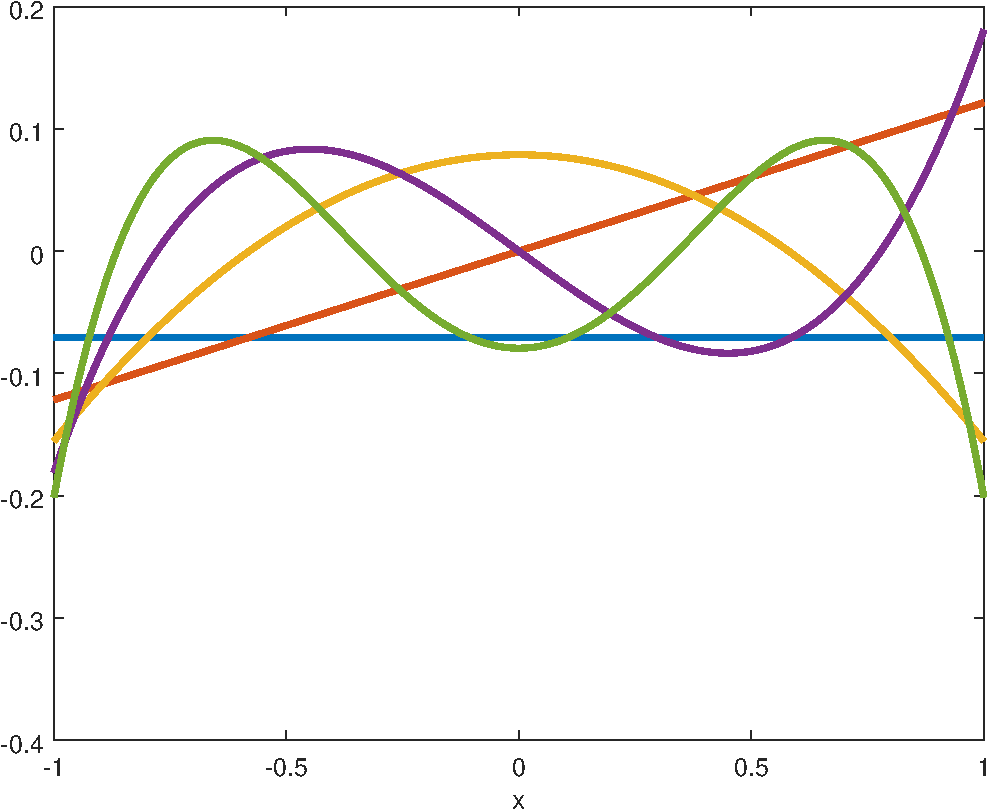
\includegraphics[width=0.5\textwidth]{figs/legendre} \quad 

\item the plot shows Legendre polynomials up to degree 4
\end{itemize}
\end{frame}


\begin{frame}{X}

\begin{itemize}
\item Y
\end{itemize}
\end{frame}

\begin{frame}{X}

\begin{itemize}
\item Y
\end{itemize}
\end{frame}

\end{document}

